\documentclass[11pt]{article}

% this is the template for an issue of the Data Engineering Bulletin
% % all packages used by any paper must be listed here
\usepackage{deauthor,times,graphicx, url, enumitem,listing ,minted}
\graphicspath{{figures/}}

% Carlos' Latex Packages
\usepackage[colorinlistoftodos]{todonotes}
% \setuptodonotes{inline}

\begin{document}
\title{Transparent Decisions: Selective Information Disclosure With Synthetic Data}
\author{
Carlos Gavidia-Calderon$^1$, Steve Harris$^2$, Markus Hauru$^1$, Carsten Maple$^1$, Iain Stenson$^1$, and \\ May Yong$^1$ \\~\\
$^1$The Alan Turing Institute \\
$^2$University College London
}
\date{\today} % Or specify a specific date
\maketitle
\begin{abstract}
There is a growing appetite to see UK's National Health Services (NHS) harness data and artificial intelligence for the public good. It is a major challenge to strike the balance between easing access to healthcare data in order to supercharge research, and maintaining the privacy of individual patients. We introduce a human-readable, risk guided approach to generating synthetic data in \todo{from?} relational databases, to meet varying requirements in terms of data fidelity, utility and appetite for disclosure risk \todo{I think risk-disclosure sounds better} .
\end{abstract}

\section{Introduction*}

Hospitals currently manage and produce large quantities of historical
patient data.
While medical staff access this data frequently for their daily duties,
other professional communities ---scientists, software engineers, or educators--- need to follow lengthy processes to be granted
access.
This process usually involves background checks, contract signing, and 
accessing data only via a highly-restricted computing environment~\cite{harris2022}.
Patient data is highly sensitive~\cite{schomerus2022}, so controls are in place to ensure patient privacy.

While protecting patient privacy is of utmost importance, limiting access to 
patient data hinders its potential.
For instance, researchers can use data to improve diagnostic accuracy, refine our understanding of diseases, or develop personalised
treatments~\cite{tucker2020}.
Patient data can be used to improve hospital productivity, when shared
with external specialists.
For example, software engineers and data scientists could develop real-time dashboards 
for tracking patients, staff, and equipment.
And, if shared with academic institutions, patient data can be used to train the next generation of clinicians and researchers.

In order to both protect user privacy \emph{and} maximise access, we can use techniques like de-identification and aggregation over the original data before handling 
it to a third party.
While these techniques provide an extra layer of privacy protection, they are not exempt from vulnerabilities~\cite{near2021}.
For example, de-identification does remove identifying information from a dataset, but data releases are still susceptible to linkage attacks.
Aggregations requires releasing only aggregate population metrics, like counts or averages, but this still leaves outliers vulnerable to identification~\cite{tucker2020}.

% Provide an overview of the challenges or problems the hospital was facing that prompted the need for a new software solution.
% Introduce the software as a solution to these challenges.
% State the objectives of the paper, including what the reader can expect to learn.
\section{Introduction}

Current mechanisms for addressing data sharing problems are necessarily \todo{I would soften the claim to ``can be'', and probably add a citation} a) time-consuming, b) linked to inadequate privacy measures protection, c) cause unnecessary friction to analysis, d) cannot be scaled to large datasets and/or e) cannot be applied to data in relational databases, a format in which many large datasets are stored.

% Therefore tools like anonymisation, pseudonymisation, trusted research environments and synthetic data generators each can provide a degree of success in enabling access to data without the contracts. However, each of these tools are limited in their own ways.

In this paper we will begin by enumerating different motivations for sharing hospital data. An understanding of motivations important because the requirements of appropriate data sharing mechanisms depend this \todo{depend on this?}. Why we want to share data decides what data needs to be shared, and this in turn enumerates the requirements to be met if the data can convincingly be shared safely. 

We will then introduce a tool for generating synthetic data requirements of a) generating datasets in relational databases b) is scale-able \todo{I think we can say scalable} c) has a process which enables transparency and accountability and d) enables the data owners to specify what exactly information to release in accordance to the risks they want to take on and the benefits they will accrue from releasing the information.

% Offer a brief history of the hospital's operations related to the challenges being addressed (anonymisation, k-means)
% Review the existing literature or previous solutions that have been tried or proposed in similar contexts, highlighting gaps or shortcomings that your software addresses (PrivLava, relational tables)
% Requirements for transparency and auditability here??
\section{Background}

\subsection{Motivations for Data Sharing}

Motivations for a hospital to share information about patient data with the public, or to analyse real patient data with external collaborators, using careful protocols meeting legal agreements include the following:

\textbf{Enhancing Research Quality and Innovation} 
Collaboration can lead to more comprehensive research studies, allowing healthcare practitioners and researchers to test hypotheses or observe trends across a broader dataset than what's available internally. This enhances the reproducibility and significance of research findings.

\textbf{Access to Specialised Expertise} 
External collaborators bring specialised knowledge and skills that complement the in-house capabilities of a hospital. For example, collaborations with methodology researchers can lead to state of the art data analysis and interpretation, thereby improving both tool development and research outcomes. Software engineers and machine learning operations (ML Ops) engineers can build customised cyber-physical infrastructure to support analysis of patient data in real time within the hospital.

\textbf{Accelerating Medical Discoveries}
By pooling resources and data between hospitals, research can proceed at a faster pace, potentially leading to quicker discoveries in disease mechanisms, treatment effectiveness, and development of new therapies or medical technologies. Sharing patient data can facilitate the recruitment of participants for clinical trials, ensuring a diverse and adequate sample size. This can be crucial in studying rare diseases or subtypes of common diseases, especially in hospitals that offer specialisations not commonly offered elsewhere in the world. 

\textbf{Expanding Research Funding Opportunities} Collaborative research often has better chances of securing funding. Funding bodies frequently encourage or require collaboration across institutions as a criterion for grants, viewing it as a way to maximise the impact of their investment.

\textbf{Benchmarking and Quality Improvement} Comparing data across institutions can help identify best practices and areas for improvement in patient care and management. This bench-marking can drive quality improvement initiatives within a hospital.

\textbf{Education and Training} Collaborations provide educational opportunities to clinical research employees at hospitals, researchers and students at universities and research institutions, exposing them to different perspectives, methodologies, and cutting-edge research through joint ventures and knowledge exchanges.

\textbf{Building Networks and Reputation} Collaborations can enhance a hospital’s reputation in the medical and scientific community. They extend the hospital’s influence and recognition, which can attract top talent and more collaborations in the future.

\subsection{Mechanisms for Data Sharing}

Hospitals enables external collaborators access to patient data through a variety of controlled, secure, and legally compliant data-sharing mechanisms. The aim of these mechanisms are to protect patient privacy while facilitating research and collaboration. 

\subsubsection{Honorary contracts for visiting researchers}

One such mechanism is via honorary contracts. Getting an honorary contract with a hospital involves a lengthy series of steps designed to formalise the relationship between an individual (often a visiting researcher) and the hospital. These contracts are generally not paid positions but provide certain privileges and responsibilities within the hospital setting. 

Typical steps for obtaining an honorary contract involve initial inquiry and application to the relevant department or clinical group at the hospital, credential verification, background and border security investigations before approval from the relevant departments can be granted. The honorary contracts can then be drafted, reviewed, and signed. The visiting researcher attends induction and training before being issued identification and necessary access to relevant records. Honorary contracts have to be monitored and reviewed regularly. 

\subsubsection{Deidentification and Anonymisation of Patient Data}
De-identification is the process of obscuring or replacing personal identifiers to prevent the direct association of data with an individual without necessarily eliminating the possibility of re-identification. As medical information is highly time-contextual, de-identified medical data will retain higher data utility if personal identifiers such as timestamps are not removed.

Anonymisation ensures that data cannot be linked back to an individual by any means. Unlike de-identification, this process is irreversible. Data has to be stripped of all identifying details, this anonymised medical data has reduced richness of data and is limited what can be learnt from it. 

Effectiveness of both de-identification and anonymization techniques is highly dependent on context, which includes the dimensionality, volume, and statistical properties of data. Other important aspects that need to be considered include which types of applications or analyses the data are to be used for, whether the data will be released publicly or with additional access control and whether the data are tabular, relational, or have longitudinal or transactional characteristics.

\subsubsection{Trusted Research Environments}

Trusted Research Environments (TREs) are an important part of the data sharing mechanisms ecosystem. TREs are the secure infrastructure and governance model that allows researchers to access and analyse data; they are often used in conjunction with other data-sharing mechanisms.

TREs play a major role in controlling the data access levels. To begin with, data access is controlled through secure authentication and authorisation mechanisms. This means that only approved researchers can access the data, and they can only access specific datasets approved for their role and research projects. Activities on TREs are closely monitored and logged.

In addition, TREs provide both physical and virtual security. Data in TREs are often stored in physically protected facilities. Virtual securities \todo{security?} measures such as firewalls, intrusion detection systems and regular penetration testing maximise protection against external threats.  Finally, to ensure no privacy leakage, data egress from TREs are restricted. Researchers can analyse data within TREs but cannot take it out.

This means that working with data within TREs is far from a comfortable experience. In order to provide security measures, computational resources can be limited and the list of approved software packages for analysis is restrictive and not easily updated. There is significant process overhead generated by the need for detailed authentication into remote machines, activity logging, monitoring and compliance checks. There is a steep learning curve in working within a TRE, new users are heavily dependent on support staff for technical assistance. Finally, the inability to egress data limits the sharing of interim findings and prevents close collaboration on ongoing data analysis. 

\subsubsection{Synthetic Data Generators}

Synthetic data generators generate datasets which mirror statistical properties of real data. There is a balance to be struck here in regards to the application of generators; synthetic data which is very similar to the real dataset (high fidelity) risk leaking information about real patients (low privacy). However, the utility of low-fidelity datasets is limited; analysis conclusions are less likely to be applicable to real data.

\begin{figure}[ht]
\centering

\includegraphics[width=0.8\linewidth]{figures/ONS.png}
\caption{Shows the range of fidelity for synthetic data. High fidelity data can result in higher utility, but also increased risk of identification.}
\label{fig:Range of fidelity for synthetic data}
\end{figure}

Figure 1 shows the range of fidelity for synthetic data. In the context of healthcare relational datasets: 

\begin{itemize}
    \item \textbf{Structurally correct datasets} has the same column names, tables and relationships as real data. 
    \item \textbf{Valid datasets} imply that the values in the synthetic dataset are correct and correct eg. date of births are valid dates. 
    \item \textbf{Plausible datasets} imply that the relationship between values are realistic eg. a patient's date of death is not before their date of birth.
    \item \textbf{Multivariate plausible datasets} implies that the values are correlated across different variables eg. a male patient like likely to be both heavier and taller than a female patient. 
    \item \textbf{Multivariate detailed datasets} are even realistic than a multivariate plausible data set, but less than a replica of the real data. An example is rows of data showing that patient with a diabetes diagnosis has more records of blood sugar readings than a patient with a broken bone.
\end{itemize}

High fidelity data is likely to be more useful (analytic valuable), but also has an increased risk of identification (disclosure risk). The three factors: a) fidelity, b) utility and c) privacy are all factors to be decided according to different use cases. 

For example, synthetic datasets for the purpose of software testing is necessarily low fidelity if access cannot be strictly controlled but it could still be useful by being only structurally correct.  Multivariate-plausible data could be sufficient for initial exploration, building pipe-lining and test modules for models. These tasks can be performed in a secure environment whose access is limited to students and researchers; these scripts ported into the hospital to be trained on real data if initial analysis is shown to be promising.

\textit{NOTE: Carsten, can I have some help here please? Some words about state of the art generators and their applications and limitations would be really useful}

\section{Use Case: Data Sharing at UCLH}

\subsection{Introduction}

This section introduces a case study to assess a hospital's requirements for making a convincing case to share data safely, and how some of those requirements can be met. 

University College London Hospitals National Health Services Foundation (UCLH NHS) Trust  is a pioneering institution within the UK, renowned for its treatment care and specialist services not widely available in other NHS Trusts. It is closely affiliated with University College London; this is a partnership that emphasises research and education, integrating medical research and teaching at the undergraduate and postgraduate levels directly into the clinical environment. 

As an institute that emphasises medical care, research and education, and as custodians of highly sensitive medical data, UCLH NHS Trust are in a position to leverage research capabilities to supercharge innovation if they can develop a process for thoughtful access to this data. However, consequences of accidentally releasing identifiable information include loss of individuals' privacy, loss of institutional prestige, as well as substantial legal fines.

UCLH NHS Trust has identified two clear motivations for exploring data sharing options in their near future; they are a) Enable Access to Specialised Expertise and b) Education and Training. 

\subsection{Problem Statement}

Machine learning (ML) infrastructure are deployed in hospitals to enable AI in healthcare delivery and administration. ML infrastructure support tasks such as structuring data from electronic health records into a format that can be used as inputs to AI algorithms, deploying image analysis and predictive analysis tools and presenting the results to health care practitioners in a timely and useful format.

To achieve these tasks, engineers who build the infrastructure need to gain an understanding of the data structures and data flow within the hospital. Researchers need to evaluate if target datasets meet their purposes for hypothesis testing, and is adequate in terms of quality and quantity. It is onerous to issue contracts to entire teams of engineers, researchers and students, but there are no other ways to share data with external collaborators. 

However, what engineers and researchers working on early stages of exploratory analysis need to gain an understanding of the data in terms of content, structure and data flow is information \textbf{about} the data, not access to individual rows of data itself. This provides us the opportunity to frame the problem as: What information can be released about sensitive data, which is maximally beneficial to engineers and researchers with minimal cost to patient privacy?

\subsection{Challenges}

\begin{enumerate}[leftmargin=*]
    \item \textbf{To generate synthetic data using statistical properties or marginals of real data.
    }
    
    Hospitals are mandated or encouraged by various information acts to release hospital information to the public. The main reasons for this is allowing insights into quality of care provided by public or insurance funds and to enable patients to make informed decisions regarding where to seek care based on hospital performance and specialisations\cite{Werner2005}. 

    The type of information that is released in the public domain include quality of care indicators, patient safety data, readmission rates and service availability. This includes data about patient outcomes, infection rates, details on specialised services, bed occupancy, Accidents and Emergency (A\&E) wait times as well as statistics on patients returning for treatment within a period of discharge. This information is published regularly and does not compromise on individual patient privacy.  

    Synthetic data generators can generate synthetic datasets which mirror statistical properties of real data. Therefore, a synthetic hospital dataset that is generated using public statistical properties will not leak patient information any more than the release of those statistical properties has, already. 
    
    \todo{At least in HSBC, they didn't even want to publish column/table names. We might need to address why it's OK in healthcare}

    \item \textbf{To generate large synthetic relational datasets.
    }
    
    Many data holders, including hospitals store patient electronic health records in relational databases. Data is often structured within complex schema that capture both single observations and time series data. These relational databases also include tables for vocabularies such as definitions of drugs, observations and diagnoses. 

    Under this challenge a minimally useful synthetic dataset must at the very least a) be structurally correct. That is, it will contain the same tables, columns, and data types, and b) meet foreign key constraints. In order to increase analytical value as shown in Figure 1, the synthetic generator will need to generate values which are valid and plausible eg. valid gender values, plausible distribution of height and weight.  A multivariate plausible dataset will have values that correlate across multiple tables eg. the correlation between gender and height are represented across the Demographic and Observation tables. 
    
    An additional complexity here is in generating synthetic time series data eg. blood pressure values every ten minutes for a patient in intensive care unit. In order to be multivariate plausible, the data needs to contain the correct frequencies for data collection as well as plausible values that depend on a patient's physiology. This is generated across multiple tables as well.  

    \item \textbf{To communicate clearly what information is being taken out from hospital data.
    }
    
    Differential privacy is the gold standard that protects individual data within a dataset while still allowing for the useful analysis of the aggregate data. However, the role of this concept when applied to synthetic data is challenging to explain. 
    
    Synthetic data is complex, people may not understand how data that does not represent real individuals still needs privacy considerations. Differential privacy is both technical and abstract and there is a struggle to understand how it offers probabilistic but not absolute guarantees. Explaining this to custodians of highly sensitive data is difficult because privacy is expected but not always technically feasible.
    
    The application of differential privacy to synthetic data compounds the explanations' complexities. However this is a important discussion, there is a necessary understanding to be achieved here because the interplay between privacy and utility governs the results of a differential-ly private synthetic data generator. The only people who can take the responsibility for managing the balance between privacy and utility are the data custodians.
\end{enumerate}

% Describe the methodology used in developing the software, including any frameworks, programming languages, or tools utilized (SSG, SQLAlchemy)
% Outline the software's architecture and components, explaining how each contributes to solving the hospital's challenges. (YAML file, sql injections)
% Discuss any innovative features or approaches used in the software's design and development.
\section{Synthetic Data Generator for Relational Databases}

\subsection{SQLSynthGen: Introduction}

SqlSynthGen (SSG) is a software package that we have written to meet the challenges described in Section 3.3. When linked to an existing relational database, SSG creates new empty database with the same schema, copies over the non-sensitive data such as vocabulary tables and finally populates it with synthetic data. 

SSG's default output dataset is structurally correct and has no disclosure risk. These are datasets that sit on the far left end of the spectrum in Figure 1. No information about the real dataset has been disclosed, beyond the structure in which they are stored. However, this can already be useful e.g. for building software testing modules and pipe-lining scripts, and can be safely released if vocabularies and schema can be shared.

However SSG can be configured to generates synthetic data which, on the Figure 1 spectrum is up to multivariate plausible. This is achieved by SSG enabling the user to define SQL statements to extract statistical properties of the real data. These values are then used to form the distributions and marginals of the synthetic data. 

SSG configuration allows dataset output to be shifted towards the right in a selective manner. The user specifies exactly which marginals are extracted from the source data, and how they are used to inform the synthetic data. SSG configuration allows for agile development with incremental fidelity improvements only as specified, with transparency, auditability, and control over privacy risk at all stages. The user can also choose to use differential privacy to protect the marginals extracted from the source data.

\subsection{SQLSynthGen: Process for Generating Synthetic Data}

\begin{figure}[ht]
\centering
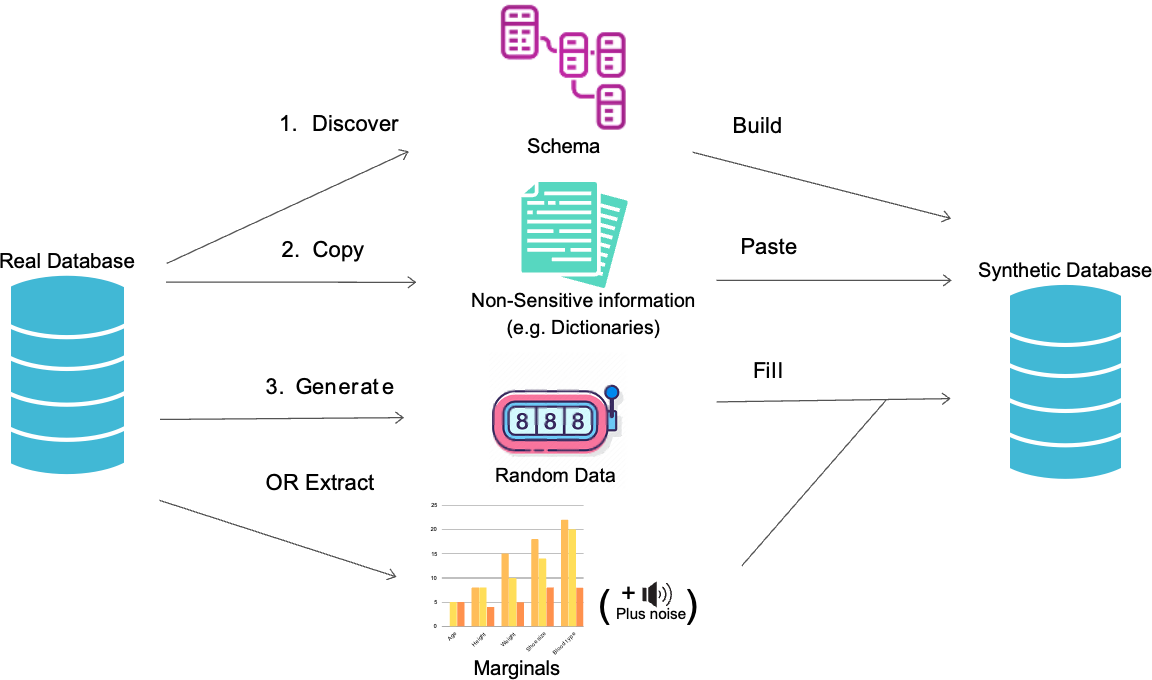
\includegraphics[width=0.8\linewidth]{figures/SSG.png}
\caption{The processes of SQLSynthGen in order}
\label{fig:Range of fidelity for synthetic data}
\end{figure}

SSG's steps for generating synthetic relational datasets as shown in Figure 2, are as follows:

\begin{enumerate}
    \item SSG discovers the schema of the real and creates a new database to store synthetic data. This new database will be populated in Step 3 below. 
    \item SSG copies over some tables entirely. This step is to maintain foreign key constraints, and is used to populate lookup tables which do not have any privacy concerns.
    \item By default, SSG populates the destination database with only structurally correct data. \item Alternatively, SSG extracts statistics from the source database to parameterise custom generators to make higher fidelity synthetic data. For example, we could extract mean height by age and gender and define some custom data generators to create a relationship between them. The user decides what is extracted and writes the custom generators as Python functions.
\end{enumerate}

For more information and tutorials about SQLSynthGen, please refer to our repository at \url{https://github.com/alan-turing-institute/sqlsynthgen}. Our repository \cite{repository} contains installation instructions, comprehensive documentation and trouble shooting guides to help get started with the software. The repository also contains a simple tutorial using a Kaggle dataset \cite{airbnb} as well as an advanced example based on the Observational Medical Outcomes Partnership (OMOP)\cite{omop}, which provides a standardised data model for observational healthcare data. 

\subsection{SQLSynthGen: Example Usage with AirBnB Relational Dataset}

The next section demonstrates the use of SSG in creating synthetic data based a publicly available AirBnB Kaggle dataset \cite{airbnb}. Install SQLSynthGen with \texttt{pip install sqlsynthgen}. To verify that the installation was successful run \texttt{sqlsynthgen --help} at the terminal, within the work directory. 

\subsubsection{Set up default configuration}

For reference in this example, let us consider that our AirBnb dataset is contained in an `airbnb` database in a local PostgreSQL instance. We want to port the schema to a new `airbnb\_synthetic` database, and populate the `airbnb\_synthetic` database with synthetic rows that mirror some of the statistical properties of the `airbnb` dataset.

First, we need to provide SSG with the connection parameters to the real dataset, using a \texttt{.env} file in listing \ref{lst:.env}.

\begin{listing}[H]
\begin{minted}[
    gobble=2,
    frame=single,
    % linenos
  ]{yaml}
    SRC_HOST_NAME=localhost 
    SRC_USER_NAME=postgres 
    SRC_PASSWORD=password
    SRC_DB_NAME=airbnb 
    DST_HOST_NAME=localhost 
    :
    DST_DB_NAME=airbnb_synthetic
\end{minted}
\caption{Example configuration for .env file"}
\label{lst:.env}
\end{listing}

We run a series of commands \mintinline{bash}{sqlsynthgen make-tables}, \mintinline{bash}{sqlsynthgen create-tables} and \mintinline{bash}{sqlsynthgen make-generators} to auto-generate two Python files. 

The first file, \texttt{orm.py}, delineates the structure of the Postgres `airbnb` dataset by mapping each table in 'airbnb' to a Python class, with table columns represented as class variables. This mapping is generated using SQLAlchemy\cite{sqlalchemy}, which is a SQL toolkit and Object-Relational Mapping (ORM) library for Python. The use of SQLAlchemy in SSG means that no further user configuration is required to describe the schema of the original dataset. 

The \texttt{orm.py} file is then used as basis to make a new `airbnb\_synthetic` Postgres database with the necessary tables, columns, and data types. Listing \ref{lst:orm.py} shows a snippet from \texttt{orm.py} which illustrates the representation of the \texttt{users} table from the `airbnb`  dataset as a Python class.

\begin{listing}[H]
\begin{minted}[
    % gobble=2,
    frame=single,
    % linenos
  ]{Python}
class User(Base):
    __tablename__ = "users"

    id = Column(String, primary_key=True)
    date_account_created = Column(Date)
    ...
\end{minted}
\caption{Postgres table `User` represented as a Python class}
\label{lst:orm.py}
\end{listing}

The second file, \texttt{ssg.py}, contains auto-generated Python code for populating each table column. This code generates default synthetic values that match the data types defined by the database schema but are not related to the actual data. The provision of human-readable code enables transparency about how each table column is populated. It can be used as a template that users can edit to incorporate different generation methods as needed.

Listing \ref{lst:ssg.py} demonstrates the auto-generated Python code for generating `id` and `date\_account\_created` values for the `User` table. `id` is assigned generic, password-like values, and `date\_account\_created` is assigned a random date value. We execute \mintinline{bash}{sqlsynthgen create-data} to populate `airbnb\_synthetic` with values generated by \texttt{ssg.py}.

\begin{listing}[H]
\begin{minted}[
    % gobble=2,
    frame=single,
    % linenos
  ]{Python}
class usersGenerator:
    num_rows_per_pass = 1

    def __init__(self, src_db_conn, dst_db_conn):
        pass
        self.id = generic.person.password()
        self.date_account_created = generic.datetime.date()
        ...
\end{minted}
\caption{A Python class for generating synthetic id and date\_account\_created values for Postgres table `User`}
\label{lst:ssg.py}
\end{listing}

\subsubsection{Copy vocabulary tables}

In this section, we demonstrate how to designate vocabulary tables so that they will be copied in their entirety, avoiding the need to generate synthetic values for them. We specify vocabulary tables in a \texttt{config.yaml}; the listing \ref{lst:vocabulary-config.yam } below denotes `countries` as a vocabulary table.

\begin{listing}
\begin{minted}[
    gobble=2,
    frame=single,
    % linenos
  ]{yaml}
    tables:
        countries:
            vocabulary_table: true
\end{minted}
\caption{A yaml section to demarcate table 'countries' as a vocabulary table}
\label{lst:vocabulary-config.yam }
\end{listing}

All values in a vocabulary table are copied to an auto-generated \texttt{.yaml} file. Listing [] shows a snippet of data from the `countries` table which has been copied to a auto-generated \texttt{countries.yaml} file.

\begin{minted}[
    gobble=2,
    frame=single,
    % linenos
  ]{yaml}
    - country_destination: AU
      destination_km2: 7741220
      destination_language: eng
        :
    - country_destination: CA
      destination_km2: 9984670
      destination_language: eng
      distance_km: 2828.1333
        :
\end{minted}

This design choice enables users to verify each value extracted from the real dataset, maximising transparency and enabling audit.

\subsubsection{Incorporate aggregate statistics}

This section shows how we incorporate aggregate statistics of real data in order to generate synthetic data that retains those statistical properties.

For example, we would like to generate normally distributed synthetic values for the users.age column, with reference to the mean and standard deviation values of the real data. SSG connects to the database and discovers requisite statistical values by running user-defined SQL statements in the \texttt{age\_stats} section of a \texttt{config.yaml} file.

\begin{minted}[
    gobble=2,
    frame=single,
    % linenos
  ]{yaml}
    src-stats:
        - name: age_stats
        query: >
        SELECT AVG(age)::float AS mean, STDDEV(age)::float AS std_dev
        FROM users
        WHERE age <= 100
    tables:
        users:
            row_generators:
              - name: airbnb_generators.user_age_provider
                kwargs:
                  query_results: SRC_STATS["age_stats"]
                columns_assigned: age
\end{minted}

Results from running these SQL statements are recorded in an auto-generated \texttt{src-stats.yaml} file. This SSG design choice enables users to access a human-readable record of what has been extracted from the real data.

\begin{minted}[
    gobble=2,
    frame=single,
    % linenos
  ]{yaml}
    age_stats:
    - mean: 36.54434029695572
      std_dev: 11.708339792587486
\end{minted}

All values extracted by SSG and placed in \texttt{src-stats.yaml} can be referenced by the Python data generators to return a distribution of values that meet those mean and standard deviation values.

\begin{minted}[
    gobble=0,
    frame=single,
    % linenos
  ]{Python}
    import random
    def user_age_provider(query_results):
    mean: float = query_results[0]["mean"]
    std_dev: float = query_results[0]["std_dev"]
    return random.gauss(mean, std_dev)
\end{minted}

\subsubsection{Build multivariate relationships across tables}

Story generators are the most complex SSG configuration option. These address generating synthetic data with correlations that bridge different tables and multiple rows.

An SSG story generator is a Python generator (an unfortunate clash of terminology: Python uses the term “generator” to refer to objects that yield multiple values in a sequence), written by the user, that yields sets of rows to be written into the synthetic database. For instance, it may first yield a row specifying a person in the users table, and then a set of multiple rows for the sessions table that specify various browsing sessions this user has had. This set of multiple rows can be related in any user-defined way eg. values increasing over time.

% \subsection{Software Design and Development}

\section{Plans for Implementation}
% Detail how the software was implemented within the hospital's existing systems and workflows. (Not yet, but plans?)
% Describe any challenges encountered during the implementation phase and how they were overcome. (Steve?)
% Discuss the training and support provided to the hospital staff to facilitate the adoption of the software. (Steve?)
% Include feedback from the hospital staff and patients, if available, to provide a comprehensive view of the software's impact. (Patient engagement group?)


\section{Discussion}
% Explore the broader implications of your findings for similar institutions or settings (any relational tables, HSBC?)
% Address any limitations of your study or software and suggest areas for future research or development. (SECURITY!!!)

\section{Conclusion}
Summarise the key points made throughout the paper, reiterating the software's role in addressing the hospital's challenges.
Reflect on the broader contributions of work to the field of healthcare IT.

\bibliographystyle{plain}
\bibliography{references}

\end{document}
